\subsection{The URDAD DSL}
\label{sec:urdadDsl}

The URDAD process is supported by a domain-specific language, the URDAD-DSL which introduces the modelling concepts required by the process and provides a concrete syntax which simplifies the specification of an URDAD model. The abstract syntax of the DSL is specified in Eclipse Ecore which is an implementation of OMG's EMOF specification with metamodel constraints specified using the \emph{Object Constraint Language} (OCL). XText was used to specify a concrete text syntax for the language. 

The URDAD DSL is not the subject of this paper. We need to, however, show aspects of the language which support quality drivers of the process.
A core aspect of URDAD as a quality driven process is the centrality of the concept of a services contract. The process requires formal requirements specifications for all services through services contracts with defined inputs and outputs, pre- and post-conditions and quality requirements and enforces decoupling of levels of granularity through these services contracts. Figure \ref{fig:contractModule} shows the contract module of the URDAD metamodel introducing the concept of a services contract.

\begin{figure*}[thbp]
  \centering
  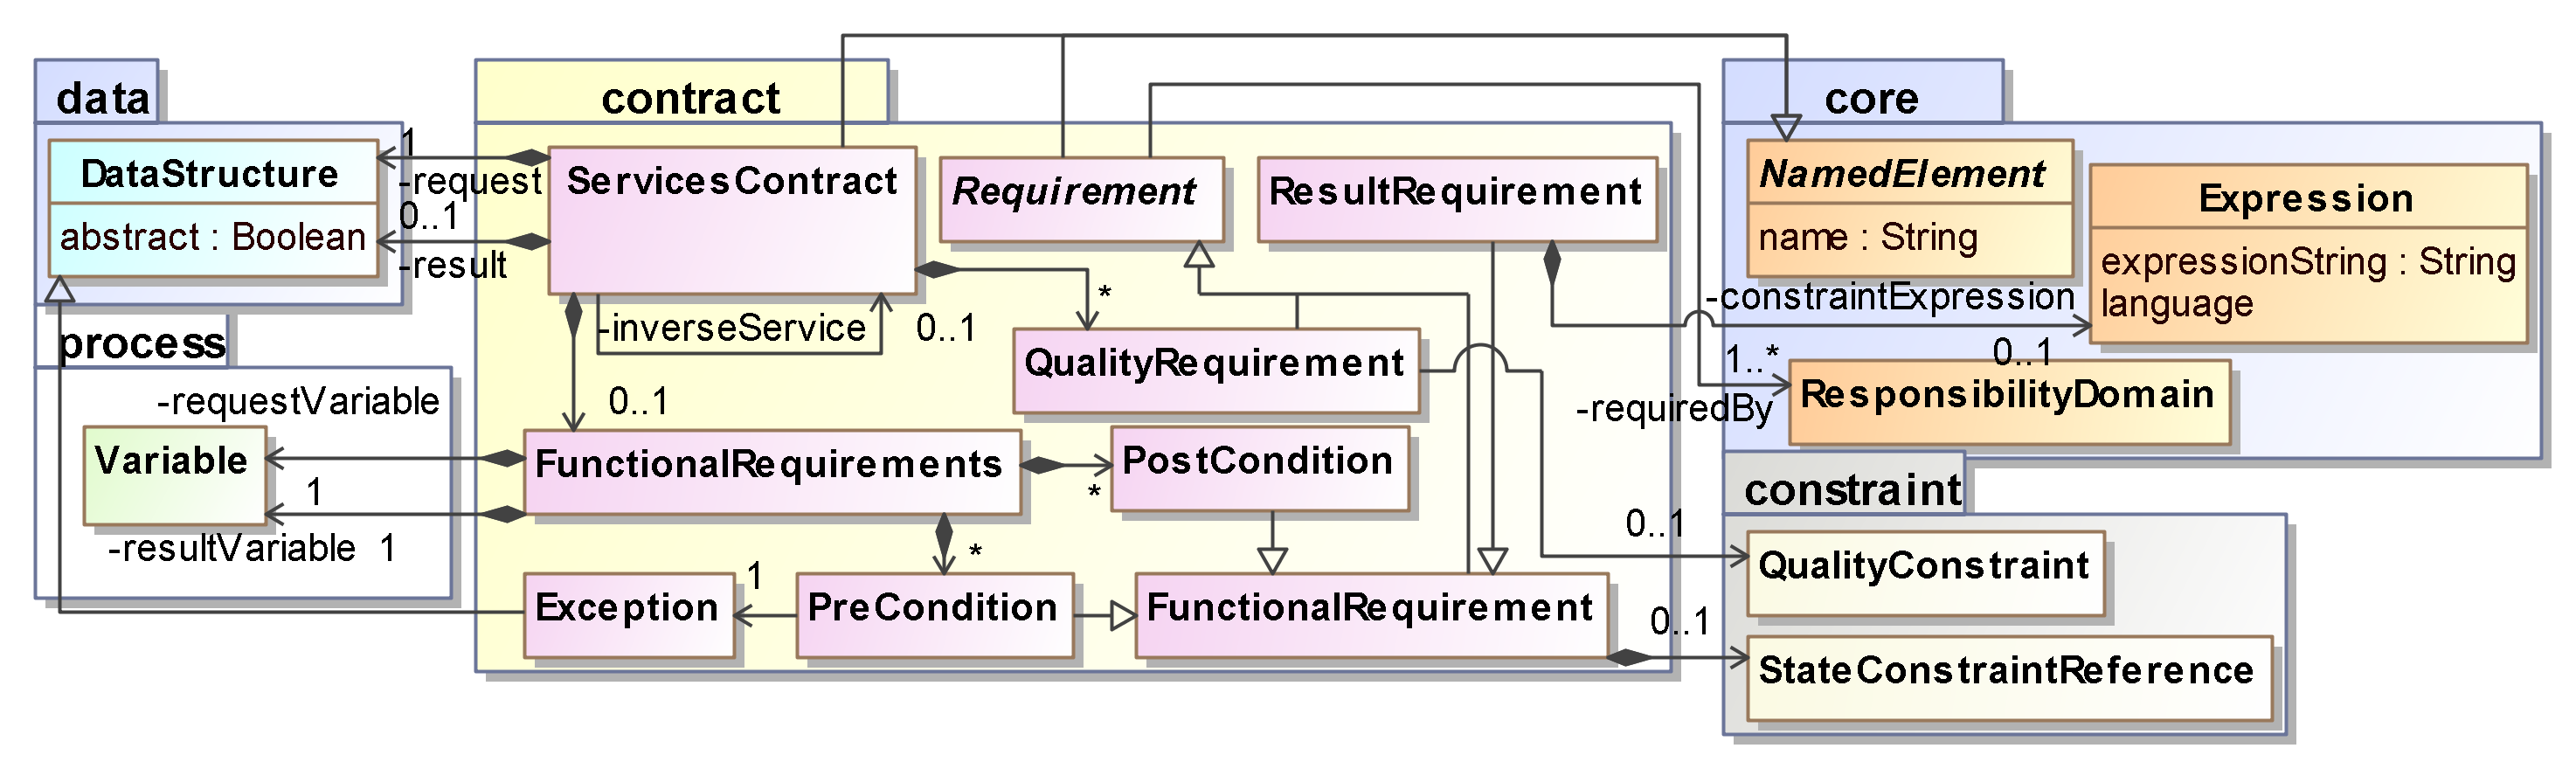
\includegraphics{contract}\\   
  \caption{The contract specification elements of URDAD}
  \label{fig:contractModule}
\end{figure*}

Note that the functional requirements (pre- and post-conditions) are linked to the stakeholders who require them. A pre-condition checks whether a constraint holds true whilst a post condition states that a constraint will old true after the service has been provided. This is illustrated in the example below which has been specified using the URDAD DSL text grammar:

\lstset{language=urdad,caption=Specifying a service contract in the textual URDAD DSL syntax.,label=contractTextSyntax}
\begin{lstlisting}[numbers=left,escapechar=|]
ServiceContract enrollForPresentation
{
 FunctionalRequirements receiving Variable enrollForPresentationRequest ofType EnrollForPresentationRequest
 {
  PreCondition enrollmentPrerequisitesMet requiredBy (TrainingRegulator Student) raises EnrollmentPrerequisitesNotSatisfiedException checks constraint enrollmentPrerequisitesForPresentationMet with ValueOf enrollForPresentationRequest
  PostCondition enrollmentProcessPerformed requiredBy (Student Client TrainingRegulator) ensures constraint studentEnrolledForPresentation          with ValueOf studentEnrolledRequest constructedUsing doSequential
  {
   create Variable studentEnrolledRequest ofType StudentEnrolledRequest
   set Query OCL:"studentEnrolledRequest.personIdentifier" equalTo Query OCL:"enrollForPresentationRequest.personIdentifier"                            
   set Query OCL:"studentEnrolledRequest.presentationIdentifier" equalTo Query OCL:"enrollForPresentationRequest.presentationIdentifier"                            
  }  
  PostCondition invoiceIssued ...
 }            
 Request DataStructure EnrollForPresentationRequest 
 {
  has identification presentationIdentifier identifying Presentation
  has identification studentIdentifier identifying Person
  has identification clientIdentifier identifying LegalEntity         
 }
 Result DataStructure EnrollForPresentationResult 
 {
  has component proofOfEnrollment ofType ProofOfEnrollment
  has component invoice ofType Invoice
  has component studyGuide ofType StudyGuide
 }
}
\end{lstlisting}

When specifying constraints, the OCL presents itself as the most widely used constraint language. It allows the specification of constraints across object graphs and also caters for the specification of message exchange constraints. On its own, it is, however, insufficient to specify constraints within a service-oriented paradigm. The reason for this is that in a services oriented paradigm, information about the environment of a service cannot be obtained by traversing an object graph. Instead one has to construct service requests which are used to query the environment and can then apply constraints on the obtained information. OCL is suited for the latter, but, being an object constraint language, it does not allow for the definition of a process which extracts the required information from the environment. The URDAD DSL provides the semantics for specifying for a constraint (used in, for example, the specification of a pre- and post-condition) a process which extracts information from the environment and then uses the OCL to apply constraints to the obtained information. 

\begin{figure*}[thbp]
  \centering
  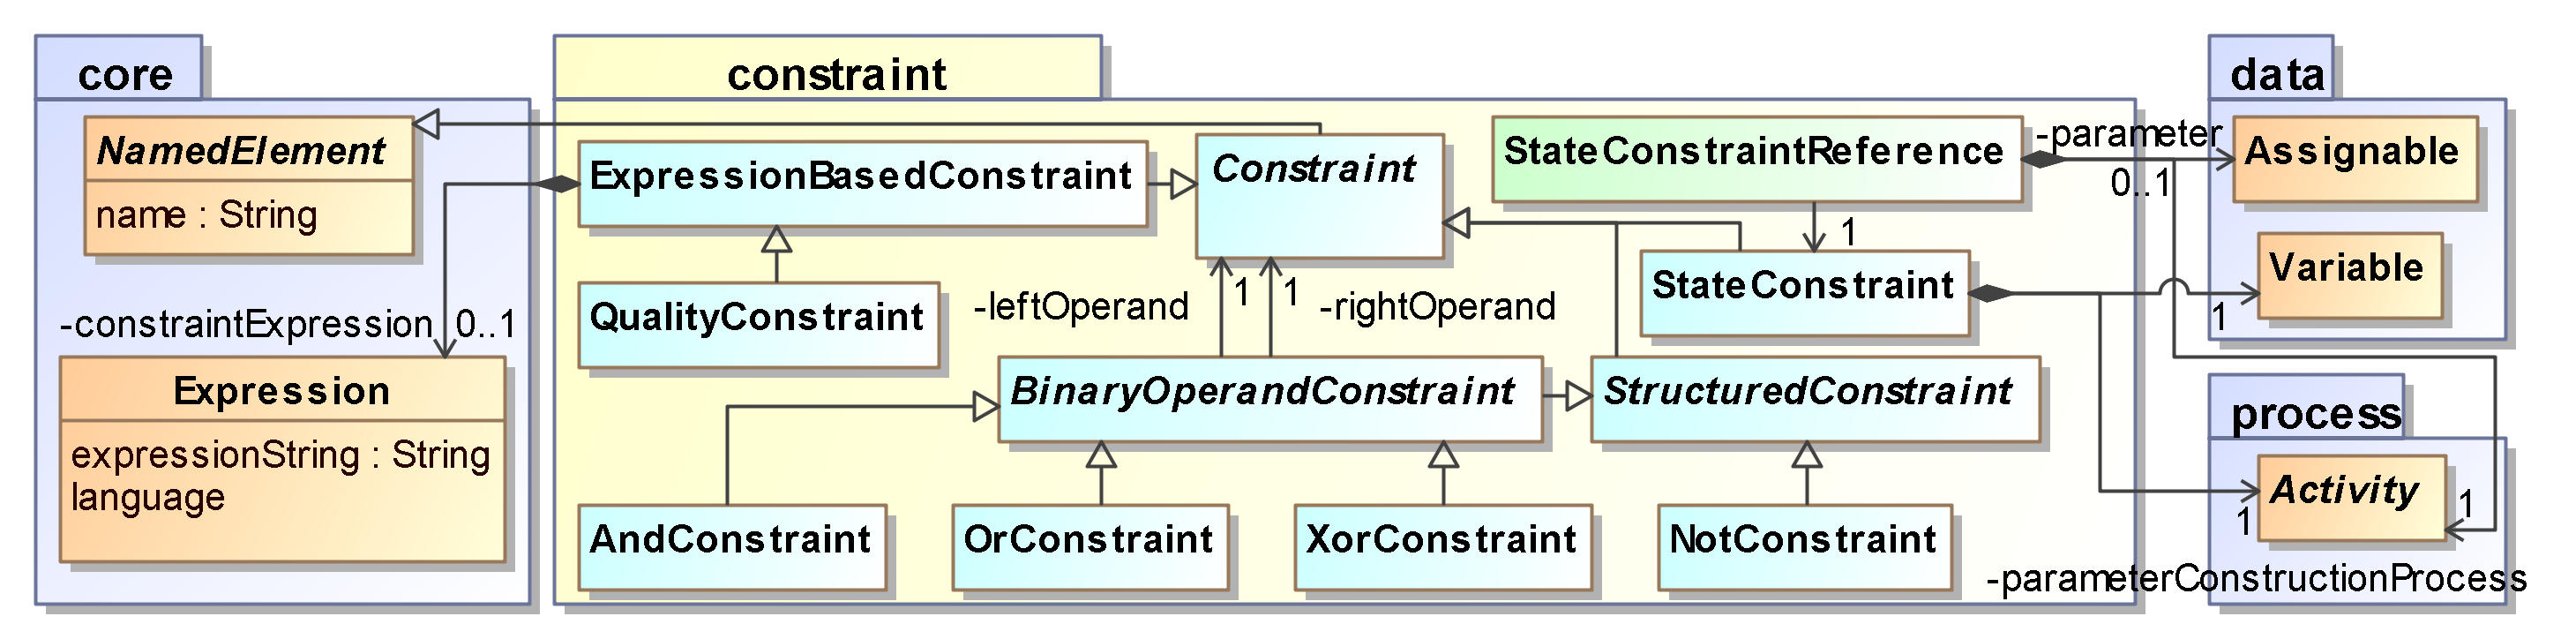
\includegraphics{constraint}\\   
  \caption{The constraint specification elements of URDAD}
  \label{fig:constraintModule}
\end{figure*}

Figure \ref{fig:constraintModule} shows the constraint module of the URDAD metamodel and below we illustrate the specification of a state constraint through a concrete example using the URDAD DSL text grammar. Note that a state constraint can be a pre-condition for several services as well as a post-condition for other services.

\lstset{language=urdad,caption=Specifying a state constraint in the textual URDAD DSL syntax.,label=constraintTextSyntax}
\begin{lstlisting}[numbers=left,escapechar=|]
StateConstraint studentEnrolledForPresentation receiving Variable enrollForPresentationRequest ofType EnrollForPresentationRequest
{
 stateAssessmentProcess doSequential
 {
  create Variable getEnrollmentsRequest ofType GetEnrollmentsRequest
  set Query OCL:"getEnrollmentsRequest.presentationIdentifier" equalTo Query OCL:"enrollForPresentationRequest.presentationIdentifier"
  requestService getEnrollments with getEnrollmentsRequest yielding Variable getEnrollmentsResult ofType GetEnrollmentsResult
 }
 Constraint OCL:"getEnrollmentsResult.enrollments.includes (enrollForPresentationRequest.personIdentifier)"
}
\end{lstlisting}

Important for the quality assessment of the process and the resultant model is the linkage enforced between services and services contracts and between activities represented by lower level service requests and functional requirements. The listing below shows how the URDAD DSL requires the specification of which abstract services are used to address which functional requirements. It then specifies a service using the services chosen to address the functional requirements. Note also that the \verb+use+ link always refers to the service specification within a services contract and not to a concrete service for which a process is specified. This enforces the decoupling between services and levels of granularity.

\lstset{language=urdad,caption=Specifying a service in the textual URDAD DSL syntax.,label=serviceTextSyntax}
\begin{lstlisting}[numbers=left,escapechar=|]
Service enrollForPresentationImpl realizes enrollForPresentation receiving Variable enrollForPresentationRequest ofType EnrollForPresentationRequest
{
 use checkStudentSatisfiesEnrollmentPrerequisites toAddress (enrollmentPrerequisitesMet)
 use issueInvoice toAddress (financialPrerequisitesSatisfied invoiceIssued) 
 use performEnrollment toAddress (invoiceIssued)
   
 Process doSequential
 {
  create Variable checkStudentSatisfiesEnrollmentPrerequisitesRequest ofType CheckStudentSatisfiesEnrollmentPrerequisitesRequest               
  set Query OCL:"enrollForPresentationRequest.studentIdentifier" equalTo Query OCL:"checkEnrollmentPrerequisitesRequest.studentIdentifier"
  set Query OCL:"enrollForPresentationRequest.presentationIdentifier" equalTo Query OCL:"checkEnrollmentPrerequisitesRequest.presentationIdentifier"
                     
  requestService checkStudentSatisfiesEnrollmentPrerequisites with checkStudentSatisfiesEnrollmentPrerequisitesRequest yielding Variable checkStudentSatisfiesEnrollmentPrerequisitesResult ofType CheckStudentSatisfiesEnrollmentPrerequisitesResult
  choice
  {
   if Constraint enrollmentMeetsPrerequisitesMet OCL:"checkStudentSatisfiesEnrollmentPrerequisitesResult.enrollmentPrerequisitesMet = true" doSequential
   {
    ...
    requestService issueInvoice with issueInvoiceRequest yielding Variable issueInvoiceResult ofType IssueInvoiceResult
    {
     on FinancialPrerequisitesNotSatisfiedException raiseException FinancialPrerequisitesNotSatisfiedException
    }
    ...
    requestService performEnrollment with enrollRequest yielding Variable performEnrollmentResult ofType PerformEnrollmentResult
          
    create Variable enrollForPresentationResult ofType EnrollForPresentationResult
    set Query OCL:"issueInvoiceResult.invoice" equalTo Query OCL:"enrollForPresentationResult.invoice"
    ...                       
    returnResult  enrollForPresentationResult
   }
   else raiseException EnrollmentPrerequisitesNotSatisfiedException
  }
 }
}                 
\end{lstlisting}

 
